\documentclass{article}
\usepackage[preprint]{neurips_2023}
\usepackage[T1]{fontenc}
\usepackage[utf8]{inputenc}
\usepackage{amsmath,amssymb,booktabs,graphicx,microtype,url}
\title{Predicting Random-Walk Cover Times on Small Graphs\\with Four Elementary Statistics}
\author{Autonomous Computational Study\\Reproducible synthetic-data experiment}
\begin{document}
\maketitle
\begin{abstract}
We test whether elementary graph statistics predict mean cover time more accurately than a universal upper bound on a small, explicitly defined synthetic benchmark. On 189 connected graphs with 6--30 vertices, a log-linear ridge model using vertex count, mean degree, maximum degree, and diameter achieves 19.9\% family-averaged absolute percentage error on held-out sizes, versus 63.4\% for a vertex-count-only model. The Monte Carlo 95\% interval is [19.7,20.2]\%, conditional on these graphs. Holding out entire graph families increases error to 29.0\%; grids and lollipops are difficult, whereas paths and barbells are easier in this suite. Each graph receives 8,192 independent simulated walks. Two generated graphs with identical input statistics have numerically exact mean cover times differing by 39.2\%, demonstrating an intrinsic limitation of the chosen features. These results support a modest empirical predictor, not a uniform accuracy guarantee or a worst-start estimate.
\end{abstract}

\section{Introduction}
Let $G=(V,E)$ be a simple, undirected, connected graph with $n=|V|$ and $m=|E|$. A simple random walk chooses a neighbor uniformly at every step. Its cover time $T$ is the first step at which all vertices have been visited, counting the initial vertex as visited at step zero. We predict
\begin{equation}
 C_U(G)=\frac1n\sum_{v\in V}\mathbb{E}_v[T],
\end{equation}
the expectation for a uniformly random initial vertex. This differs from the frequently studied worst-start quantity $C_{\max}(G)=\max_v\mathbb{E}_v[T]$.

Classical work gives general bounds and connections to hitting times \citep{aleliunas1979,lovasz1993,feige1995}. The finite bound $C_U\leq C_{\max}\leq 2m(n-1)$ follows by traversing a spanning tree and summing edge commute times, each at most $2m$. Such a bound provides a guarantee, but may be a poor numerical estimate. We ask whether a few elementary statistics offer better empirical predictions, and whether success transfers between graph families. Our contribution is a compact, reproducible experiment with explicit simulation uncertainty, family-specific failures, and an example where the selected statistics cannot distinguish different cover times. We use the supplied classical references as background and do not conduct a literature search for existing solutions to this prediction problem.

\section{Methods}
\paragraph{Predictors.}
Set $\bar d=2m/n$, $\Delta=\max_v d_v$, and $D=\operatorname{diam}(G)$. We fit
\begin{equation}
 \log\widehat C=\beta_0+\beta_n\log n+\beta_d\log\bar d+
 \beta_\Delta\log\Delta+\beta_D\log D.
 \label{eq:model}
\end{equation}
Training-fold means and population standard deviations standardize the four log features. Ridge regression minimizes the sum of squared log residuals plus $\|\beta\|_2^2$ in standardized coordinates; the intercept is unpenalized. The penalty is fixed at one, without tuning. We exponentiate predictions directly, without a residual correction. Each training graph has equal weight. A second model uses only $\log n$, with the same fitting procedure. We also score $2m(n-1)$ as a numerical baseline, recognizing that it is a guarantee rather than a fitted estimator. We omit $m$ as a separate regressor because $\log m=\log n+\log\bar d-\log2$. Graph labels are not model inputs. The features require at most all-source breadth-first searches for diameter, trivial at these sizes.

\paragraph{Monte Carlo estimation and checks.}
For each graph we simulate $R=8{,}192$ walks, independently choosing each initial vertex uniformly. Walks run to completion with no truncation. The label is the sample mean $\bar T$, with standard error $s/\sqrt R$ and approximate 95\% interval $\bar T\pm t_{R-1,.975}s/\sqrt R$. Seeds derive from master seed 20261027; graphs and walks have separate streams. The CPU simulator uses an unbiased bounded-integer sampler. We retain every trajectory length and the full graph edge lists.

We check the simulator against known values for paths, cycles, stars, and complete graphs, and against subset-state equations for one six-vertex graph per family. For visited set $S$ and current vertex $v\in S$, these equations are
\begin{equation}
 h(S,v)=1+\frac{1}{d_v}\sum_{w\sim v}h(S\cup\{w\},w),\qquad h(V,v)=0.
\end{equation}
Solving in decreasing set size gives $C_U=n^{-1}\sum_v h(\{v\},v)$. The 33 distinct graph checks have maximum standardized discrepancy 2.42; 30 of 33 means include the reference value in their nominal 95\% intervals. This is a diagnostic, not a simultaneous coverage guarantee. Median and maximum relative Monte Carlo interval half-widths over all 189 graphs are 1.19\% and 2.54\%.

\section{Experiments and results}
\paragraph{Graph suite and evaluation.}
We use $n\in\{6,10,14,18,22,26,30\}$. At every size we generate one path, cycle, star, complete graph, grid, lollipop, and barbell; ten connected Erd\H{o}s--R\'enyi (ER) graphs; and ten uniformly sampled labeled trees (via Pr\"ufer sequences). Thus there are 189 graphs. ER uses $p=\min(0.6,2\log n/n)$ with rejection until connected. A grid consists of the first $n$ row-major lattice sites of width $\lfloor\sqrt n\rfloor$, including horizontal and vertical edges. A lollipop has a clique of size $\lfloor2n/3\rfloor$ joined to a path containing the remaining vertices. A barbell has two cliques of size $\lfloor n/3\rfloor$ and a connecting path with $n-2\lfloor n/3\rfloor$ internal vertices. These choices form a small benchmark, not a random sample of all connected graphs.

In the \emph{size interpolation} protocol, sizes 14 and 26 are held out in every family: 135 training graphs and 54 test graphs. In \emph{leave-one-family-out} (LOFO) evaluation, each family is tested on a model trained on the other eight families, across all seven sizes. Any training graph isomorphic to a held-out graph is also removed (three removals for the path fold, three for the tree fold, and two for the barbell fold). Evaluation averages absolute percentage error within each family, then averages those nine values equally. Consequently, the larger ER and tree samples do not dominate the reported metric, although they do receive more total training weight. The two protocols have different test sets and are not a paired estimate of a distribution-shift effect.

To propagate Monte Carlo error through both fitting and scoring, we divide each graph's walks into 64 batches of 128. We independently resample batches within every graph, recompute means, refit all models, and rescore, for 300 bootstrap replicates (seed 20261028). Reported metric intervals are the 2.5th and 97.5th percentiles. They quantify simulation uncertainty conditional on this fixed graph suite; they do not quantify uncertainty over possible graph populations.

\begin{table}[t]
\centering
\caption{Family-averaged absolute percentage error (\%). Brackets give Monte Carlo 95\% intervals, including refitting. The bound is scored as an estimate only.}
\label{tab:main}
\begin{tabular}{lrr}
\toprule
Method & Size interpolation & Leave one family out\\
\midrule
Universal bound & 1700.4 [1694.0, 1707.4] & 1529.5 [1526.1, 1532.7] \\
$n$ only & 63.4 [63.0, 63.7] & 69.3 [69.1, 69.5] \\
Four statistics & 19.9 [19.7, 20.2] & 29.0 [28.8, 29.2] \\
\bottomrule
\end{tabular}

\end{table}

\paragraph{Accuracy and family dependence.}
Table~\ref{tab:main} shows that four statistics substantially improve average prediction over both baselines in this suite. The interpolation model, expressed in original feature units, is approximately
\begin{equation}
 \widehat C=0.523\,n^{0.815}\bar d^{0.032}\Delta^{0.693}D^{1.251}.
\end{equation}
These are fitted associations, not a scaling law; correlated inputs and the sampling design limit coefficient interpretation. Full-precision coefficients are included in the results archive.

Interpolation errors for paths, cycles, and barbells are 6.2\%, 6.8\%, and 4.0\%, respectively. Errors for grids and lollipops are much larger: 46.4\% and 44.1\%. In LOFO, paths and barbells remain near 5\%, but grids reach 49.4\% [48.8,50.1] and lollipops 57.8\% [57.3,58.3]. Stars, complete graphs, and ER graphs also deteriorate, reaching 36.2\%, 40.8\%, and 41.1\%. Thus poor transfer is not confined to obvious bottleneck graphs. Figure~\ref{fig:results} shows the substantial family dependence. The bound's particularly large aggregate error partly reflects complete graphs, whose interpolation error exceeds 11,000\%; the learned $n$-only baseline provides a more demanding comparison.

\begin{figure}[t]
\centering
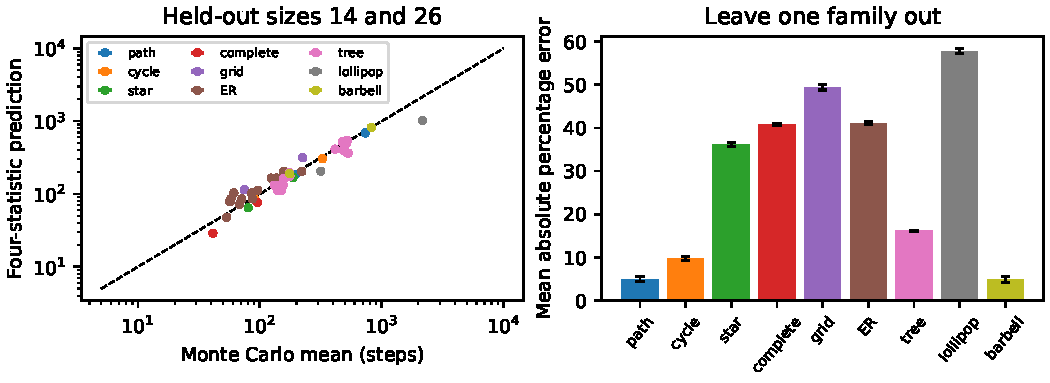
\includegraphics[width=\linewidth]{results/results.pdf}
\caption{Left: four-statistic predictions at held-out sizes; horizontal bars are Monte Carlo 95\% intervals, often smaller than the markers. The dashed line is equality. Right: per-family LOFO error with conditional Monte Carlo bootstrap intervals.}
\label{fig:results}
\end{figure}

\paragraph{Identical features, different cover times.}
Among generated nonisomorphic graphs, IDs 37 and 39 have identical $(n,m,\bar d,\Delta,D)=(6,10,10/3,5,2)$. Their simulated means are 16.22 [16.01,16.42] and 22.25 [21.85,22.65] steps. An additional subset-state calculation gives 16.0871 and 22.3954 steps, a 39.2\% difference. Their edge lists are archived. This pair was selected after examining feature collisions and is descriptive, not a prespecified significance test. Nonetheless, the state equations demonstrate that these statistics do not determine the target: any predictor assigning the same value to both must incur at least $(22.3954-16.0871)/(22.3954+16.0871)=16.4\%$ relative error on one. A richer regression on the same inputs cannot remove this ambiguity.

\section{Discussion and limitations}
The answer is affirmative for average accuracy on this benchmark, with clear restrictions. The four-statistic model is useful for the sampled paths, cycles, trees, and barbells, but its errors are too large to call it uniformly reliable. Diameter and degree extrema capture some variation, while missing details of access to rarely visited regions. The lollipop results are consistent with such missing information; the accurate barbell predictions show that a bottleneck alone does not imply failure. The experiment does not establish a causal explanation of these family differences.

The suite excludes odd sizes, sizes below six, weighted or directed graphs, and many possible structures. Deterministic families supply only two interpolation test graphs each. Random families use one sampling regime and ten draws per size; narrow Monte Carlo intervals do not imply broad generalization. We assess uniform-start means only: neither these predictions nor their intervals estimate worst-start cover times or individual-walk tails. Ridge regularization, unweighted training, and direct exponentiation may influence relative error. No feature or hyperparameter search was performed. Additional structural descriptors and family-balanced training are possible follow-ups, but remain untested here.

All computation uses CPU only. Simulation, exact checks, and saving data take about seven seconds; the complete experiment, bootstrap, and figures take about twenty seconds on this environment. The release includes source, pinned dependencies, raw trajectories, graph seeds and edges, predictions, validation results, and this paper's LaTeX source with the unmodified official NeurIPS 2023 style. It can be rerun with \texttt{make reproduce} after installing the documented dependencies.

\bibliographystyle{plainnat}
\bibliography{references}
\end{document}
